\documentclass{article}
\usepackage{lmodern}
\usepackage[T1]{fontenc}
\usepackage{shapepar}
\usepackage{microtype}
\usepackage{lipsum}
\usepackage{pgfplots}
\pgfplotsset{compat=1.9}
\usepackage{tikz}
\usetikzlibrary{calc,fit,intersections,folding}
\usepackage{pstricks-add}
\usetikzlibrary{arrows.meta,angles,arrows,quotes,backgrounds,calc,shapes}


\newcommand{\clrone}{blue}
\newcommand{\clrtwo}{red}

\begin{document}
\thispagestyle{empty}

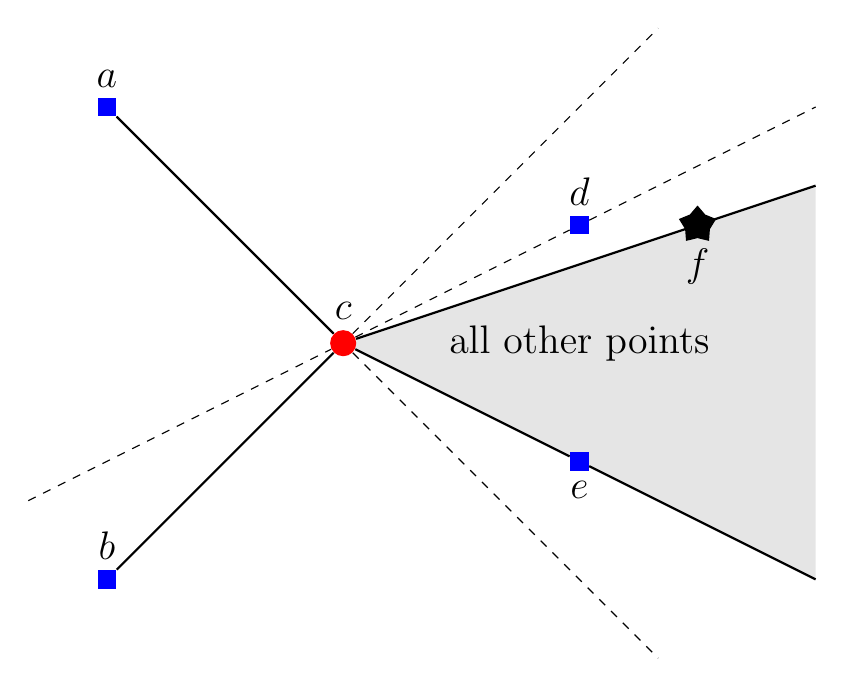
\begin{tikzpicture}


    \fill[opacity = 0.1] (3,0) -- (9,-3) -- (9,2) -- cycle;
    
    \node[fill, \clrone, label=\Large$a$] (a) at (0,3) {};
    \node[fill, \clrone, label=\Large$b$] (b) at (0,-3) {};
    \node[fill, circle, \clrtwo, label=\Large$c$] (c) at (3,0) {};
    \node[fill, \clrone, label=\Large$d$] (d) at (6,1.5) {};
    \node[fill, \clrone, label=below:\Large$e$] (e) at (6,-1.5) {};
    \node[fill, star, label=below:\Large$f$] (f) at (7.5,1.5) {};

    \node at (6,0) {\Large all other points};

    \draw[thick] (a) -- (c) -- (e) -- (9,-3);
    \draw[thick] (b) -- (c);
    \draw[dashed] (-1,-2) -- (c) -- (d) -- (9,3);
    \draw[thick] (c) -- (9,2);
    \draw[dashed] (a) -- (c) -- (7,4);
    \draw[dashed] (a) -- (c) -- (7,-4);

    
\end{tikzpicture}


\end{document}